\setchapterimage[6cm]{chapter/oblast_of_Russia/Flag_maps_of_the_subjects_of_Russia.png}
\chapter{Regions of Russia}
\label{ch:oblast-of-Russia}
This article is devoted to the study of the most important properties of 
the object <<The Subjects of Russia>>. Using the implementation of SPARQL-queries, 
data about the number of instances of the <<Oblast of Russia>>, about the number of 
all currently existing subjects of the Russian Federation (oblast of Russia, republics, 
federal city of Russia, the region, autonomous okrug, autonomous regions, former 
administrative-territorial units) were received, the graph of neighboring subjects 
of the Russian Federation and countries was constructed, and the map with the population 
of certain subjects of the Russian Federation was drawn. Moreover, it was considered the 
task about fullness of property <<shares border with>>. Also, fields with properties in the 
Wikidata were replenished. Reader will get acquainted with computer treatment of Wikidata 
and visualization of information about Russian districts.

\label{question:q_subjects_of_Russia_3}
\marginnote{Which entity's flag is in question:
<<The flag of this subject is a rectangular panel with a width-to-length ratio of 2:3, red in color with a two-sided image in the upper corner of the main element of the coat of arms of this subject, which is deployed to the shaft of \href{https://en.wikipedia.org/wiki/Saint_George}{Saint George}. See the answer~\ref{answer:subjects_of_Russia_3} on the page~\pageref{answer:subjects_of_Russia_3}.}

\section{Instances of the object <<Oblast of Russia>>}

To build a list of all regions of Russia, we will need an object 
\wdqName{<<oblast of Russia>>}{835714} and the property \wdProperty{31}{<<instances>>}
(query~\protect\ref{lst:oblast-of-Russia}).

\begin{lstlisting}[ language=SPARQL, 
                    caption={\href{https://w.wiki/4D2W}{List of all regions of Russia}\protect\footnotemark},
                    label=lst:oblast-of-Russia,
                    texcl 
                    ]
# List of oblasts of Russia
SELECT ?region ?regionLabel
WHERE
{
  ?region wdt:P31 wd:Q835714. # instance of "oblast of Russia"
  SERVICE wikibase:label { bd:serviceParam wikibase:language "en"}
}
\end{lstlisting}%
\footnotetext{48 records were received in 2017 and 46 records in 2021. Link to SPARQL query: \href{https://w.wiki/4D2W}{https://w.wiki/4D2W}}

In Wikidata, has the most properties in Russia and in the world \wdqName {Leningrad}{2191} and \wdqName{Kaliningrad region}{1749}, by 43 properties \autocite{Russia_prowd}. The number of properties for Russia and the world is the same, since both for Russia and for the world are the same objects.

The regions of Russia with the least number of properties according to ProWD data were: \href{http://www.wikidata.org/entity/Q3129 }{Oryol region} (31 properties), \href{http://www.wikidata.org/entity/Q3178 }{Kursk region} (31 properties), \href{http://www.wikidata.org/entity/Q5851 }{Novosibirsk region} (32 properties).

\section{Subjects of the Russian Federation}

Let's build a list of all the subjects of Russia. To do this, select the following objects in Wikidata: republics, territories, regions, cities of federal significance, autonomous regions and autonomous districts (query~\protect\ref{lst:subjects-of-Russia}).

\marginnote[2.0cm]{Objects used in SPARQL queries:
\begin{itemize}
	\item\wdqName{<<Oblast of Russia>>}{835714};
	\item\wdqName{<<Republic of Russia>>}{41162};
	\item\wdqName{<<Federal city of Russia>>}{183342};
	\item\wdqName{<<Krai of Russia>>}{831740};
	\item\wdqName{<<Autonomus oblast of Russia>>}{309166};
	\item\wdqName{<<Autonomus okrug of Russia>>}{184122};
	\item\wdqName{<<Former administrative-territorial unit>>}{19953632}.
\end{itemize}
Property used \wdProperty{31}{<<instances>>}
}

\begin{lstlisting}[ language=SPARQL, 
                    caption={\href{https://w.wiki/4D2S}{List of all subjects of Russia}\protect\footnotemark},
                    label=lst:subjects-of-Russia,
                    texcl 
                    ]
# List of `instances of` "subjects of Russia" 
SELECT ?subject ?subjectLabel ?typeLabel
WHERE
{  
  VALUES ?type {wd:Q835714   # Oblast of Russia
                wd:Q41162    # Republic of Russia
                wd:Q183342   # Federal city of Russia
                wd:Q831740   # Krai of Russia
                wd:Q309166   # Autonomus oblast of Russia
                wd:Q184122}  # Autonomus okrug of Russia
  ?subject wdt:P31 ?type.  # Selecting the type of object
  SERVICE wikibase:label { bd:serviceParam wikibase:language "en"}
}
\end{lstlisting}%

\footnotetext{85 records were received in 2017 and 86 records in 2021. Link to SPARQL query: \href{https://w.wiki/4D2S}{https://w.wiki/4D2S}. In 2021, the federal city of Baikonur was added to the list of subjects on the lease of the complex <<Baikonur>>.}

To build the script ~\protect\ref{lst:subjects-of-Russia} and to verify the results obtained, the following information is needed:
\begin{itemize}
\item According to the Constitution of the Russian Federation, Russia consists of 85 subjects - republics, territories, regions, cities of federal significance, autonomous regions, autonomous districts.
  \item This task does not take into account subjects that are not currently part of the Russian Federation (for example, \wdqName{Chita region}{182902}), because they are not instances of objects \wdqName{<<Oblast of Russia>>}{835714}, \wdqName{<<Republic of Russia>>}{41162}, \wdqName{<<Federal city of Russia>>}{183342}, \wdqName{<<Krai of Russia>>}{831740}, \wdqName{<<Autonomus oblast of Russia>>}{309166}, \wdqName{<<Autonomus okrug of Russia>>}{184122}, and belong to the object \wdqName{<<Former administrative-territorial unit>>}{19953632}. (We get 86 objects after executing a SPARQL query. Listing ~\protect\ref{lst:subjects-of-Russia}). 
  \item According to category data <<\href{https://ru.wikipedia.org/wiki/Subjects of the Russian Federation}{Subjects of the Russian Federation}>> There are 85 subjects of the Russian Federation on the Russian Wikipedia.
  \item According to category data <<\href{https://ru.wikipedia.org/wiki/en:Federal_subjects_of_Russia}{Federal subjects of Russia}>> There are also 85 subjects of the Russian Federation on the English Wikipedia.
\end{itemize}

\section{Neighboring entities}

Let's construct a graph of neighboring subjects of Russia by the property \wdProperty{47}{shares border with} (query~\protect\ref{lst:sharesBorderWith-area-of-Russia}).

\label{question:q_subjects_of_Russia_1}
\marginnote{Name the region of Russia located in the north-west of Russia and formed in \num{1920}. It borders the Leningrad, Vologda, Arkhangelsk and Murmansk regions. It also borders Finland to the west.
Select the flag of this region among the following flags. See the answer \ref{answer:subjects_of_Russia_1} on page~\pageref{answer:subjects_of_Russia_1}.}

\begin{marginfigure}[1.0cm]
{
	\setlength{\fboxsep}{0pt}%
	\setlength{\fboxrule}{1pt}%
	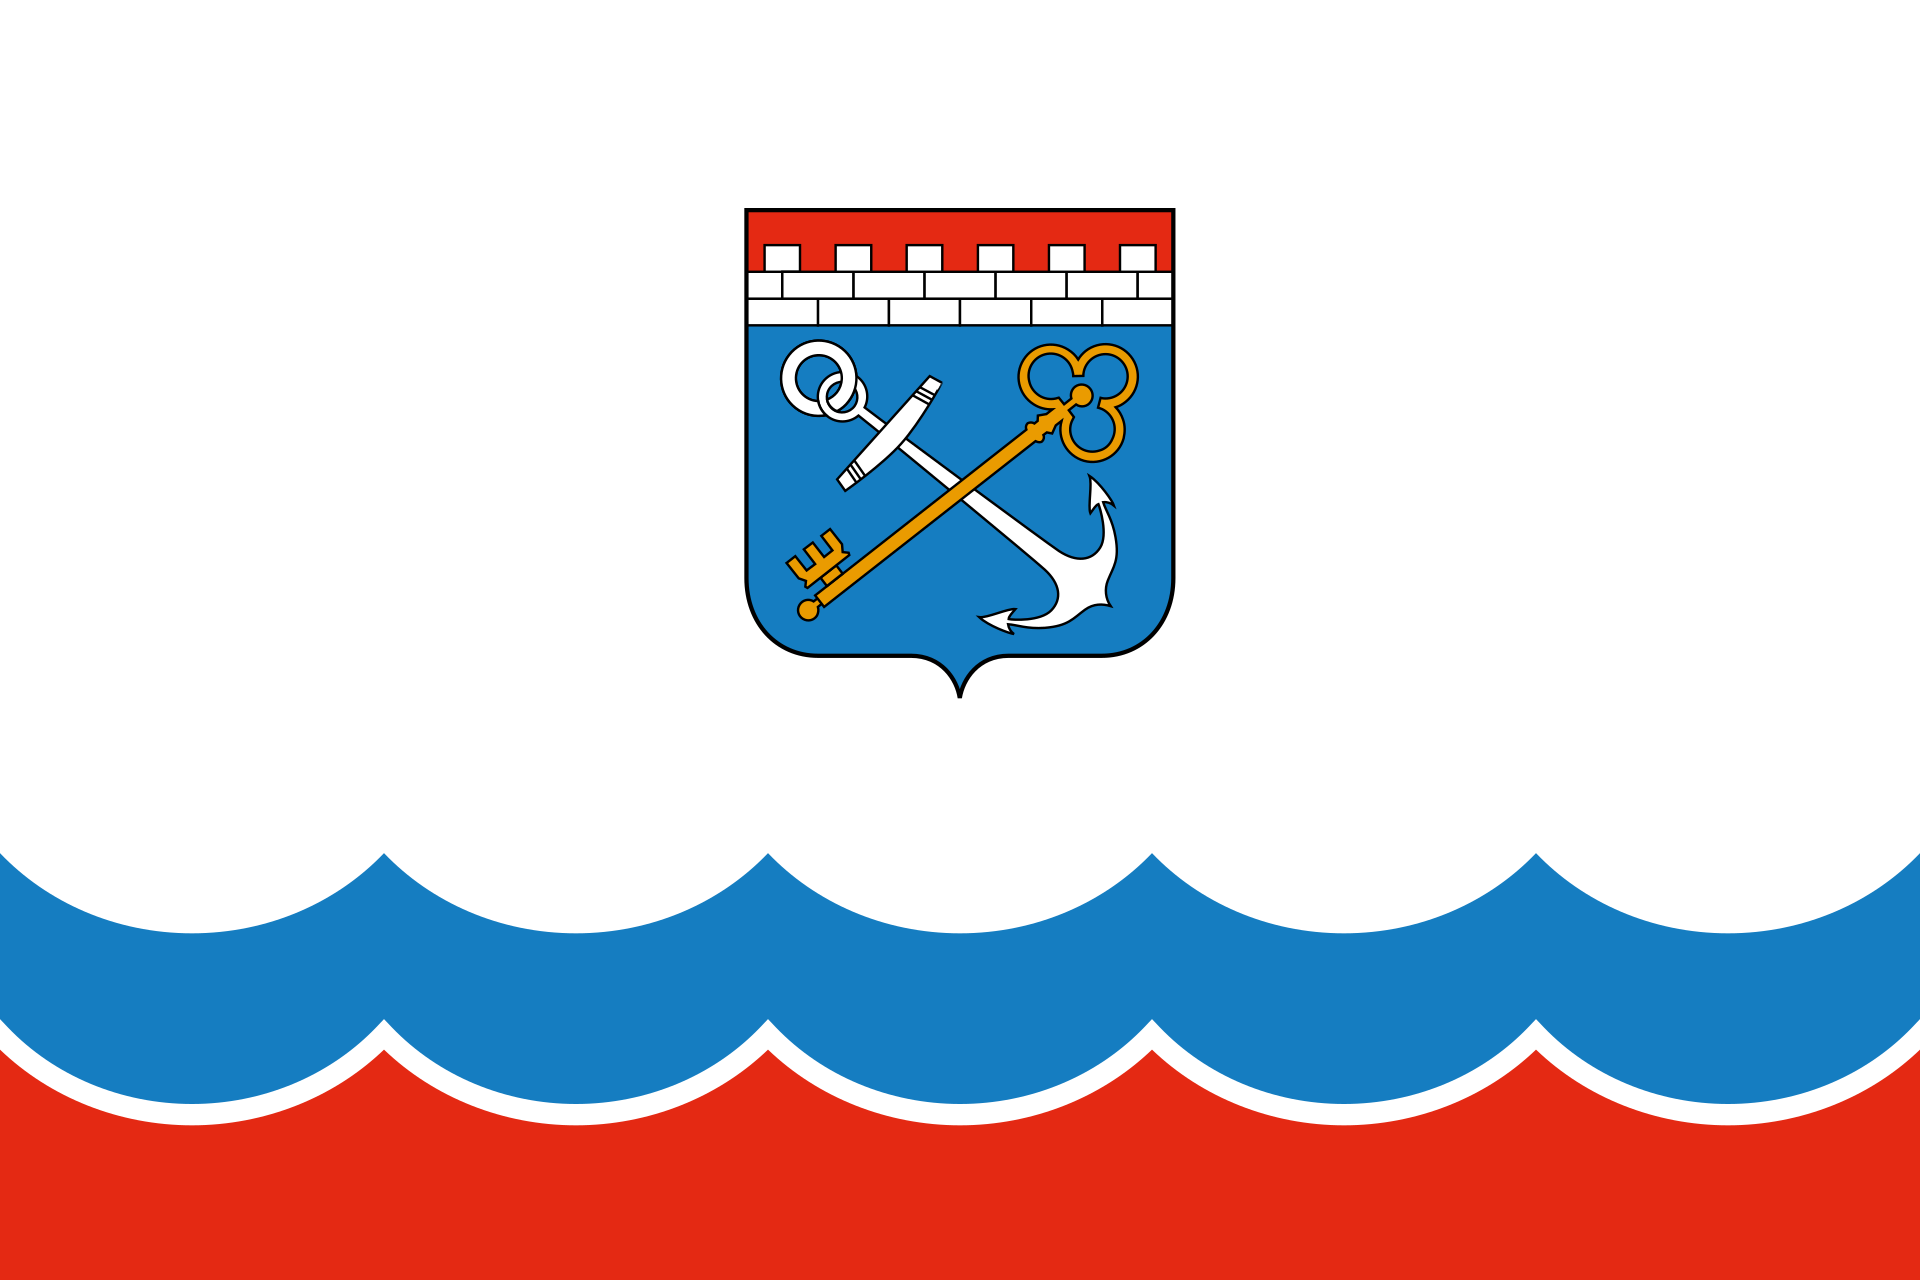
\includegraphics[width=0.8\linewidth]{"chapter/oblast_of_Russia/Flag_of_Leningrad_Oblast.png"}
}
\caption [Flag of the Leningrad region, Russia.]{Flag of the Leningrad region, Russia.}%
\label{fig:Flag_of_Leningrad_Oblast}%
\end{marginfigure}
\begin{marginfigure}[6.0cm]
{
	\setlength{\fboxsep}{0pt}%
	\setlength{\fboxrule}{1pt}%
	
\includegraphics[width=0.8\linewidth]{"chapter/oblast_of_Russia/Flag_of_Moscow_oblast.png"}
}
\caption [Flag of the Moscow region, Russia.]{Flag of the Moscow region, Russia.}%
\label{fig:Flag_of_Moscow_oblast}%
\end{marginfigure}
\begin{marginfigure}[11.0cm]
{
	\setlength{\fboxsep}{0pt}%
	\setlength{\fboxrule}{1pt}%
	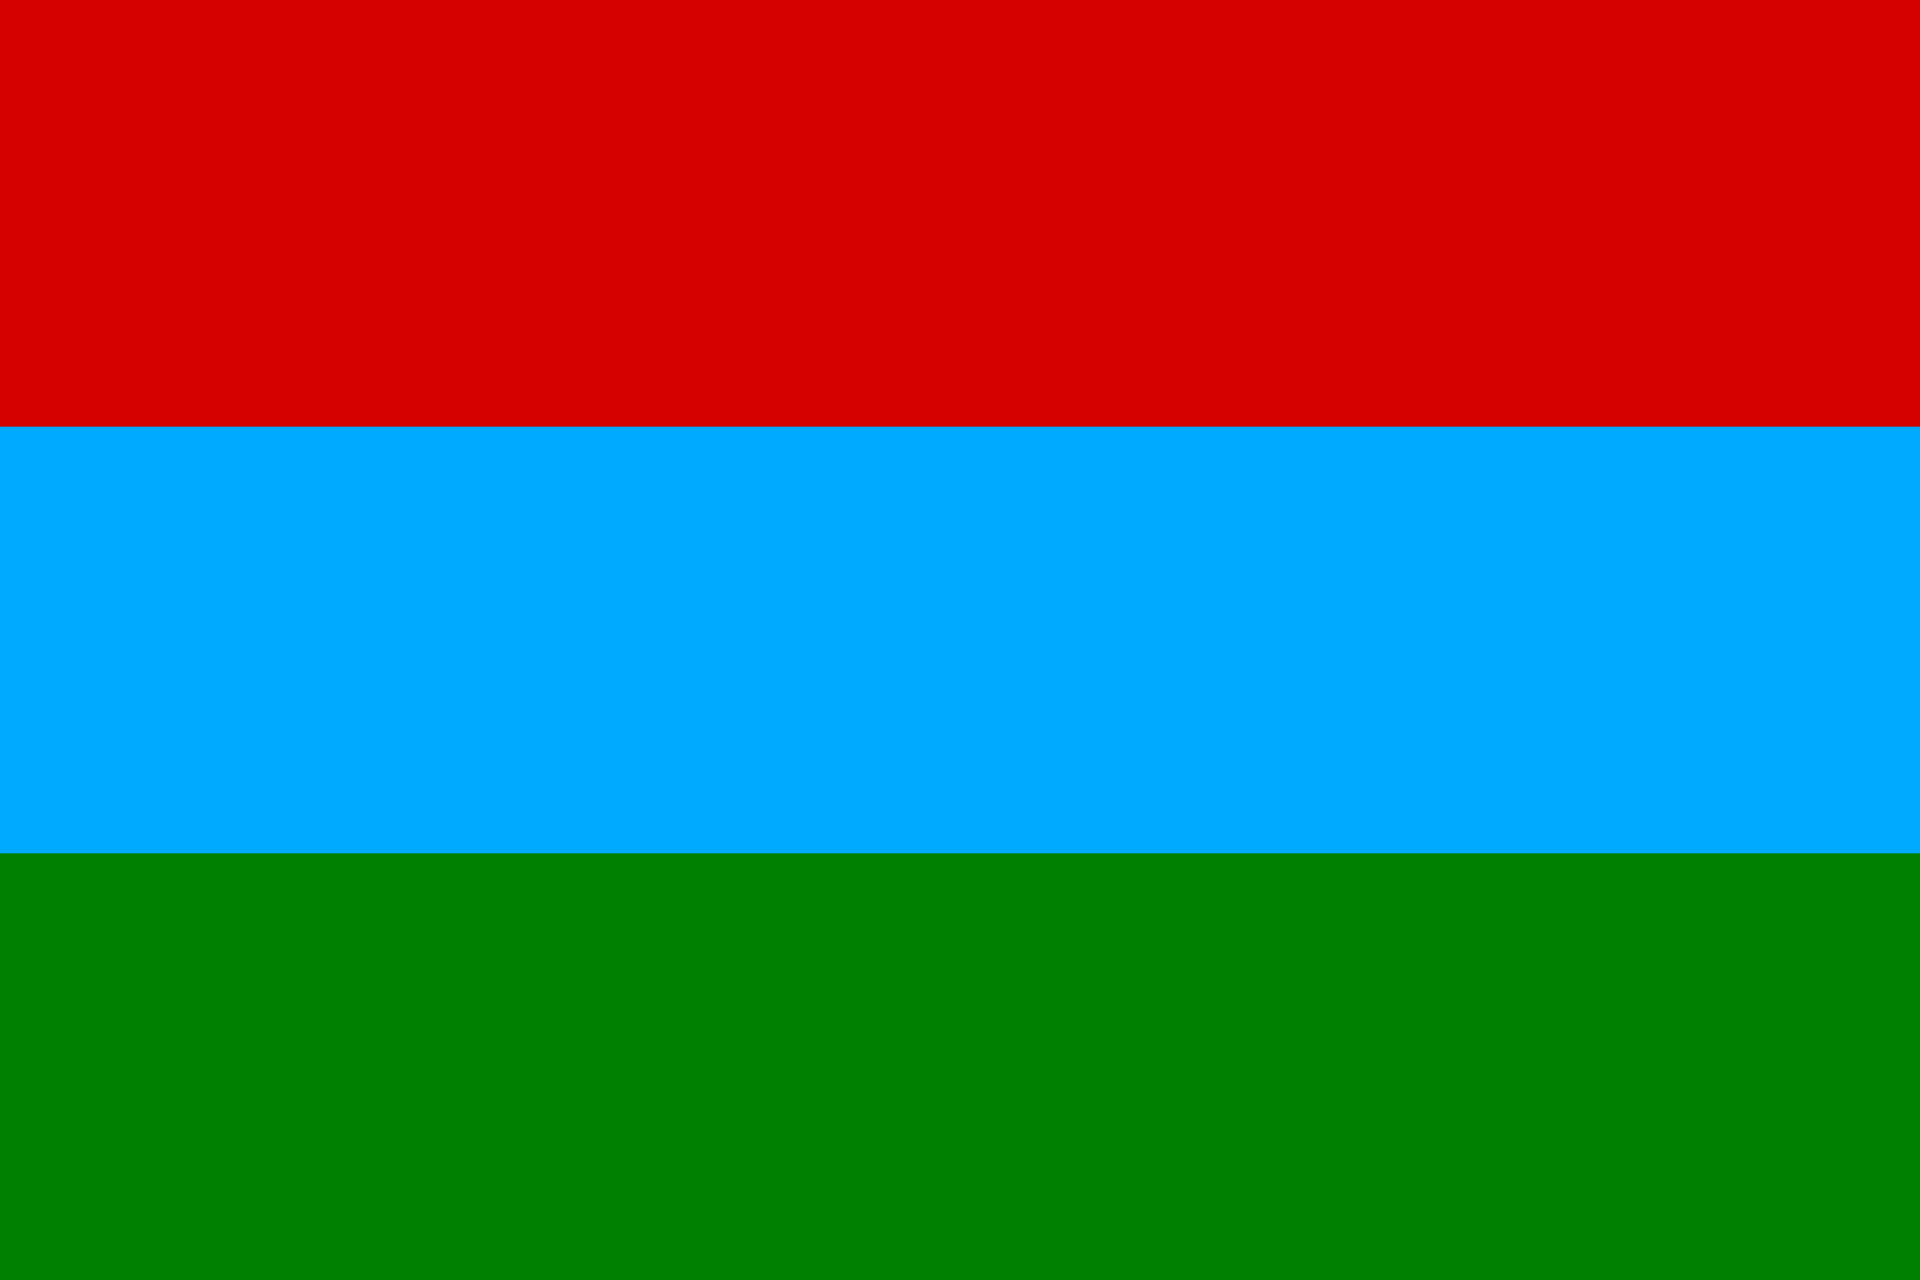
\includegraphics[width=0.8\linewidth]{"chapter/oblast_of_Russia/Flag_of_Karelia.png"}
}
\caption [Flag of Karelia, Russia.]{Flag of Karelia, Russia.}%
\label{fig:Flag_of_Karelia}%
\end{marginfigure}
\begin{marginfigure}[16.0cm]
{
	\setlength{\fboxsep}{0pt}%
	\setlength{\fboxrule}{1pt}%
	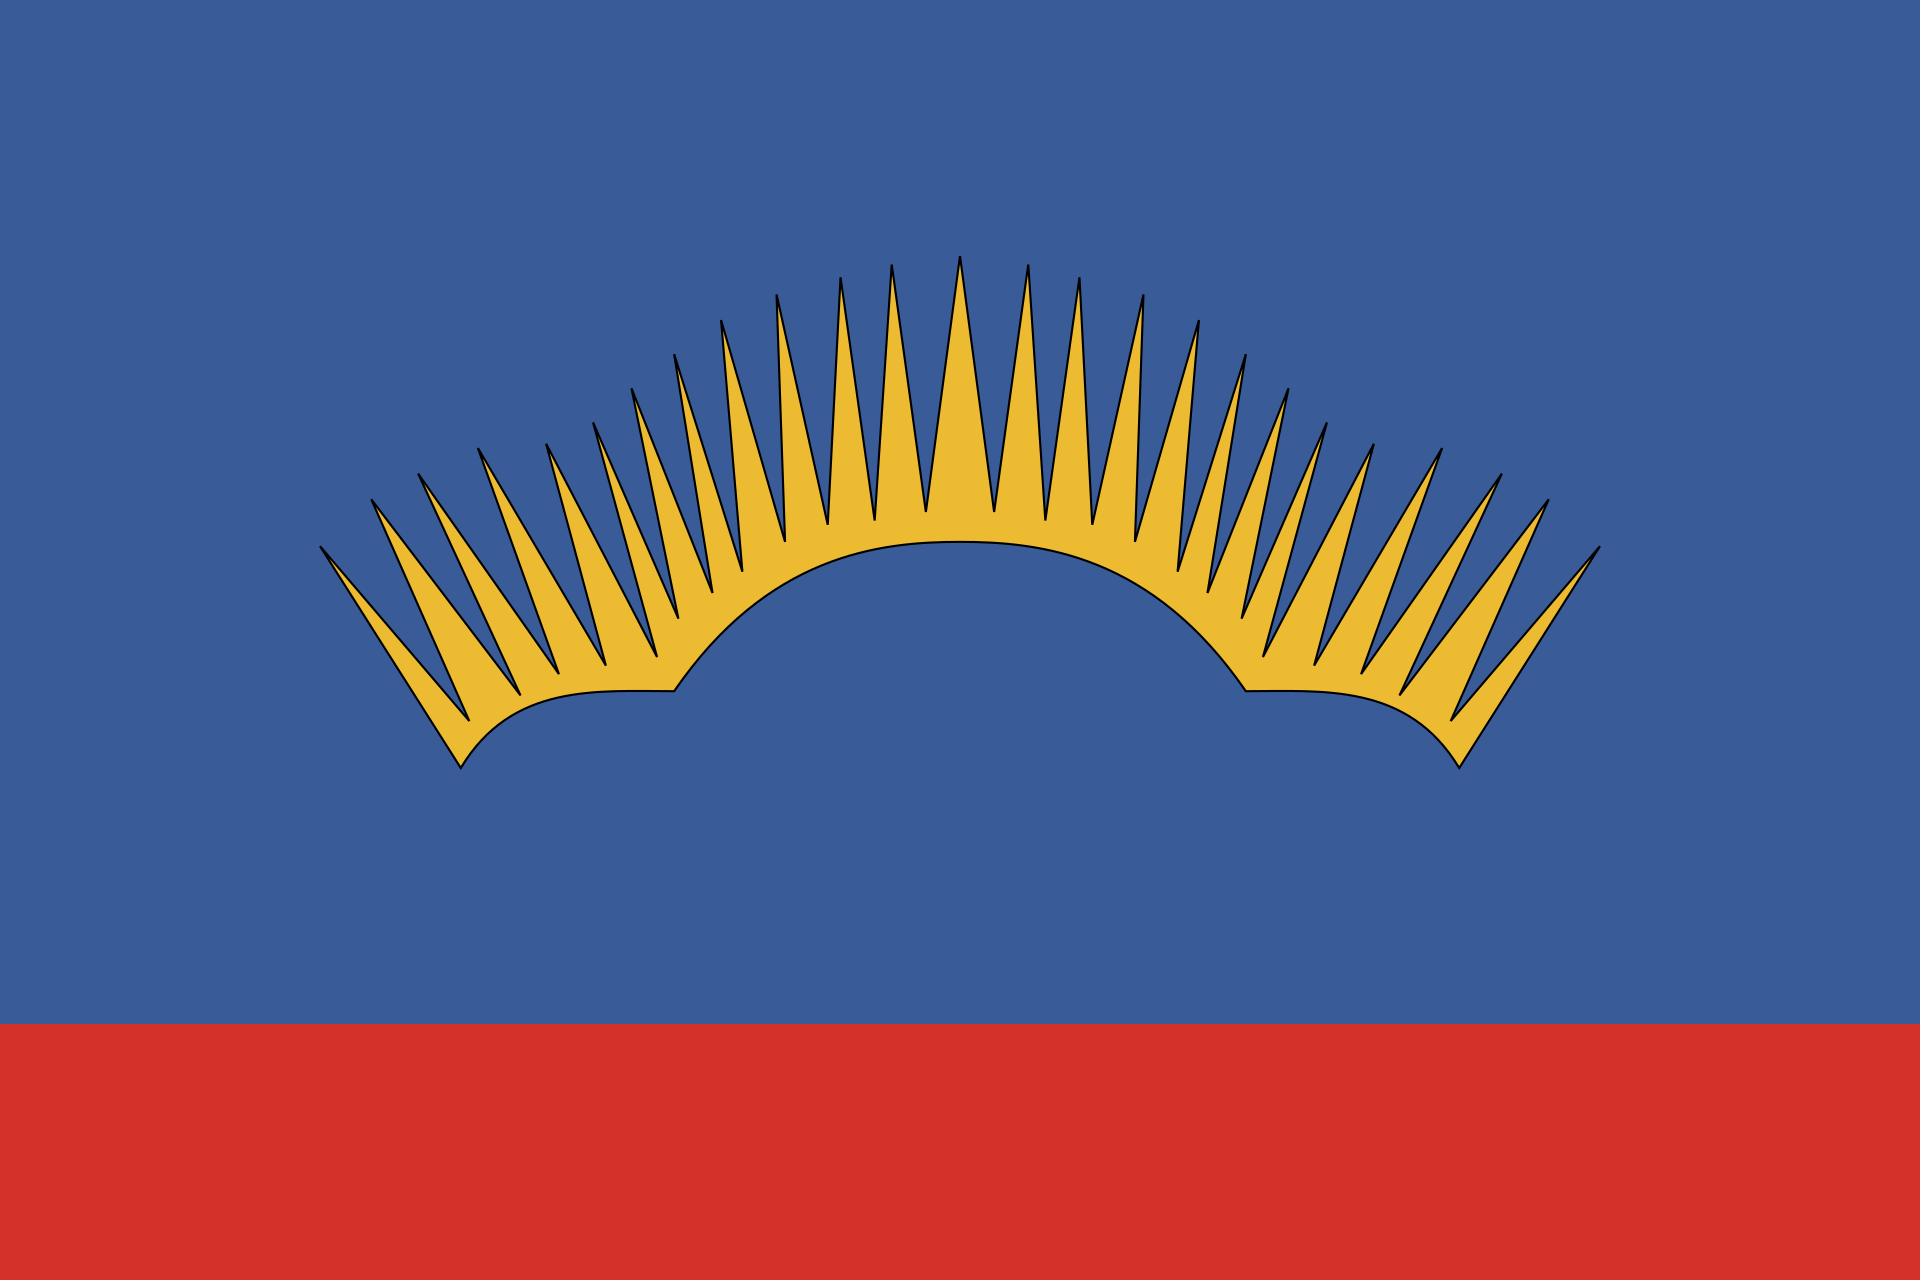
\includegraphics[width=0.8\linewidth]{"chapter/oblast_of_Russia/Flag_of_Murmansk_Oblast.png"}
}
\caption [Flag of the Murmansk region, Russia.]{Flag of the Murmansk region, Russia.}%
\label{fig:Flag_of_Murmansk_Oblast}%
\end{marginfigure}

\lstset{numbers=left, firstnumber=1, frame=single}
\begin{lstlisting}[ language=SPARQL, 
                    caption={\href{https://goo.su/9ZUj}{Graph of neighboring subjects of Russia}\protect\footnotemark},
                    label=lst:sharesBorderWith-oblast-of-Russia,
                    texcl 
                    ]
# Graph of subjects of Russia "shares border with". 
#defaultView:Graph
SELECT * WHERE {
 {
   SELECT ?subject ?subjectLabel ?rgb ?subjects ?subjectsLabel 
   WHERE {
     SERVICE wikibase:label 
            { bd:serviceParam wikibase:language "en". }
     VALUES ?type {
       wd:Q835714 wd:Q41162 wd:Q183342
       wd:Q831740 wd:Q309166 wd:Q184122
     }
     ?subject wdt:P31 ?type.
   }
 }
 UNION
 { ... }
 UNION
 {
   SELECT ?subject ?subjectLabel ?rgb ?subjects ?subjectsLabel 
   WHERE {
     SERVICE wikibase:label 
            { bd:serviceParam wikibase:language "en". }
     VALUES ?type {
       wd:Q835714 wd:Q41162 wd:Q183342
       wd:Q831740 wd:Q309166 wd:Q184122
     }
     ?subjects wdt:P31 ?type.
     ?oblast wdt:P31 wd:Q835714; wdt:P47 ?subjects.
     
     BIND(IF(?oblast != "", "e87b7b", 
                    IF(?rgb != "", ?rgb, "FFFFFF")) AS ?rgb)
     BIND(IF(?oblast != "", ?oblast, ?subjects) AS ?subject)
     BIND(IF(?oblast != "", ?oblastLabel, 
                    ?subjectsLable) AS ?subjectLable)
   }
 }
}
\end{lstlisting}%

\footnotetext{467 records were received in 2017 and 482 records in 2021. Link to SPARQL query: \href{https://goo.su/9ZUj}{Graph of neighboring subjects of Russia}}

Using the \textit{BIND} command (lines 31--35), we write the value to a variable, provided that the variable responsible for subjects of a certain type is non-empty. For example, in lines 31--32, a color is written to the variable \text{?rgb}, provided that \textit{?oblast} is not empty. At the same time, if the variable \textit{?rgb} already contains a value, then we leave it to exclude color mashing.

The number of records received is formed by adding the number of neighboring territories for all subjects of Russia. The result of the script~--- is a graph displaying neighboring subjects. Moreover, different types of subjects have vertices of different colors, for example, the republics are ~--- green, and the edges are~--- blue. Part of the graph is shown in Fig.~\ref{fig:sharesBorderWith-oblast-of-Russia-Kaliningrad-fig}.

%\begin{fullwidth}
\begin{figure*}[h]
	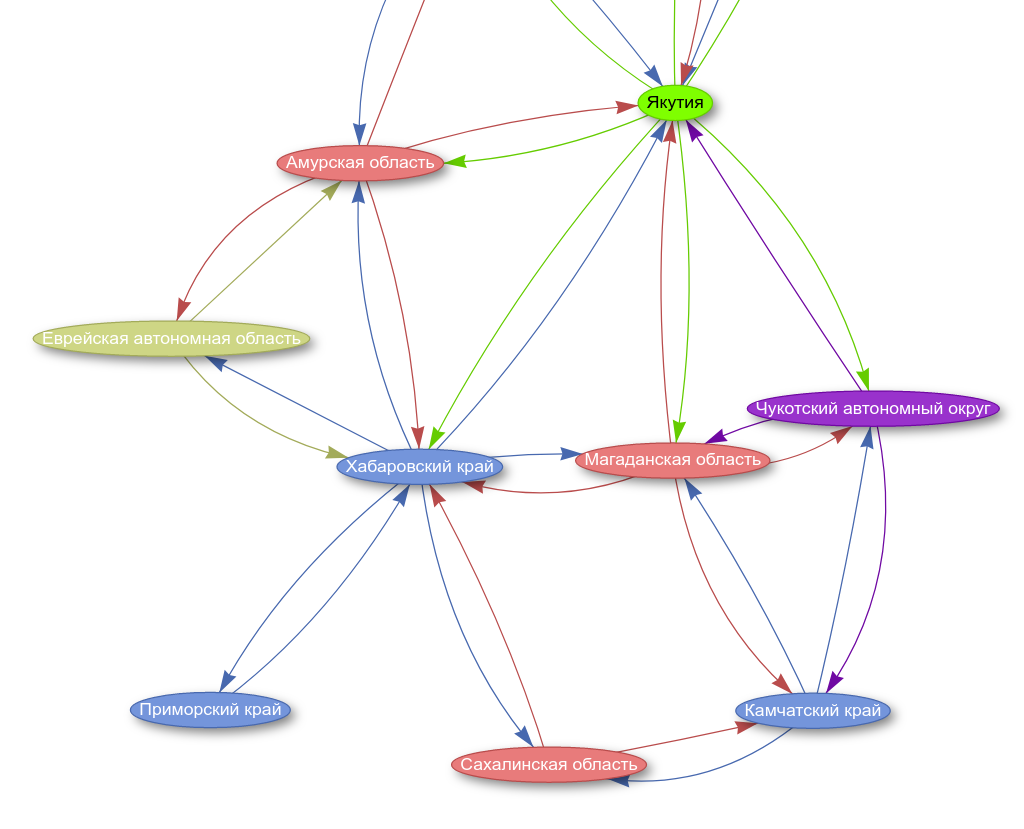
\includegraphics[width=\textwidth]{./chapter/oblast_of_Russia/Graph_Subjects_of_Russia_Siberia_and_the_Far_East_2021.png}
	\caption[Graph of the subjects of Russia. Kaliningrad, 2021.]{Regions of Russia in Siberia and the Far East for 2021. A fragment of the graph of neighboring subjects of Russia, built according to the query~\protect\ref{lst:sharesBorderWith-oblast-of-Russia}.
	Republics~--- green peaks (Yakutia).
	Autonomous Okrugs~--- purple peaks (Chukotka Autonomous Okrug).
	Edges~--- blue peaks (Khabarovsk Krai).
	Areas~--- pink peaks (Amur region).
	Autonomous regions~--- green-colored peaks (Jewish Autonomous Region).}%
      \label{fig:sharesBorderWith-oblast-of-Russia-Kaliningrad-fig}%
\end{figure*} 
%\end{fullwidth}

\newpage
\subsection{Completeness of Wikidata}

Let's build a list of subjects of Russia with an empty property \wdProperty{47}{shares border with} (borders with) (query~\protect\ref{lst:sharesBorderWith-empty-area-of-Russia}), that is, we will try to find such subjects that do not border with anyone.

\label{question:q_subjects_of_Russia_2}
\marginnote[2.0cm]{Which of the following subjects are currently part of the Russian Federation, and which are not:
\begin{itemize}
  \item Republic of Adygea;
  \item Kamchatka Krai;
  \item Chita region;
  \item Chukotka Autonomous Okrug.
\end{itemize}
See the answer \ref{answer:subjects_of_Russia_2} on page~\pageref{answer:subjects_of_Russia_2}.
}

\lstset{numbers=left, firstnumber=1, frame=single}
\begin{lstlisting}[ language=SPARQL, 
                    caption={\href{https://w.wiki/4bLL}{List of subjects of the Russian Federation with an empty property \wdProperty{47}{shares border with}}\protect\footnotemark},
                    label=lst:sharesBorderWith-empty-oblast-of-Russia,
                    texcl 
                    ]
# List of `subjects of Russia`~without `shares border with`. 
SELECT 
    ?subject ?subjectLabel 
    ?sharesBorderWith ?sharesBorderWithLabel
WHERE
{
  VALUES ?type {wd:Q835714   # Oblast of Russia
                wd:Q41162    # Republic of Russia
                wd:Q183342   # Federal city of Russia
                wd:Q831740   # Krai of Russia
                wd:Q309166   # Autonomus oblast of Russia
                wd:Q184122}  # Autonomus okrug of Russia
  
  ?subject wdt:P31 ?type.
  
  FILTER EXISTS {?subject wdt:P17 wd:Q159; wdt:P31 ?type}
  
  MINUS { ?subject  wdt:P47 [] } . #Shares border with 
  SERVICE wikibase:label { bd:serviceParam wikibase:language "en"}
}
\end{lstlisting}%
\footnotetext{Received 0 records in 2017 and 0 records in 2021. Link to SPARQL query: \href{https://w.wiki/4bLL}{https://w.wiki/4bLL}}

Using the \textit{FILTER} command (line 16), we exclude objects that are not located on the territory of Russia. Then, using \textit{MINUS} (line 20), we select objects whose property \wdProperty{47}{<<shares border with>>} is not filled.

Thus, the \wdProperty{47}{<<shares border with>>} property is filled in on Wikidata for all subjects of Russia.

\section{Population of individual subjects of the Russian Federation}

Let's mark the subjects of the Russian Federation on the map, dividing them into six groups by population. Subjects belonging to the same group will be displayed on the map in the same color.

For the query (listing~\protect\ref{lst:map}), we need the properties \wdProperty{625}{<<coordinates>>} and \wdProperty{1082}{<<population>>}.

\index{Graph!Map!Map of the population of Russia}

\begin{lstlisting}[ language=SPARQL, 
                    caption={\href{https://w.wiki/4bLQ}{Map of the population of Russia}\protect\footnotemark},
                    label=lst:map,
                    texcl 
                    ]
# Map of `population` "subject of Russia"
# Version 2021
#defaultView:Map
SELECT DISTINCT ?subject ?subjectLabel ?population ?coord ?layer
{
  {
    { ?subject wdt:P31 wd:Q835714 } UNION  # Oblast of Russia
    { ?subject wdt:P31 wd:Q41162 } UNION  # Republic of Russia
    { ?subject wdt:P31 wd:Q183342 } UNION  # Federal city of Russia
    { ?subject wdt:P31 wd:Q831740 } UNION  # Krai of Russia
    { ?subject wdt:P31 wd:Q309166 } UNION # Autonomus oblast 
                                                        of Russia
    { ?subject wdt:P31 wd:Q184122 } # Autonomus okrug of Russia
  }   
  ?subject wdt:P625 ?coord; wdt:P1082 ?population.
  
  BIND(
    IF(?population < 500000, "< 500000",
    IF(?population < 1000000, "500000 - 1000000",
    IF(?population < 3000000, "1000000 - 3000000",
    IF(?population < 8000000, "3000000 - 8000000",
    IF(?population < 10000000, "8000000 - 10000000",
    "> 10000000")))))
    AS ?layer).
  
  SERVICE wikibase:label { bd:serviceParam wikibase:language "en"}
}
ORDER BY ?population
\end{lstlisting}%

\footnotetext{Received \num{85} records in 2017 and \num{86} records in 2021. Link to SPARQL query: \href{https://w.wiki/4bLQ}{https://w.wiki/4bLQ}}

The result of the script (listing~\protect\ref{lst:map}) is shown in the figure~\ref{fig:SubjectsRussiaMap}.

%\begin{fullwidth}
\begin{figure*}[h]
	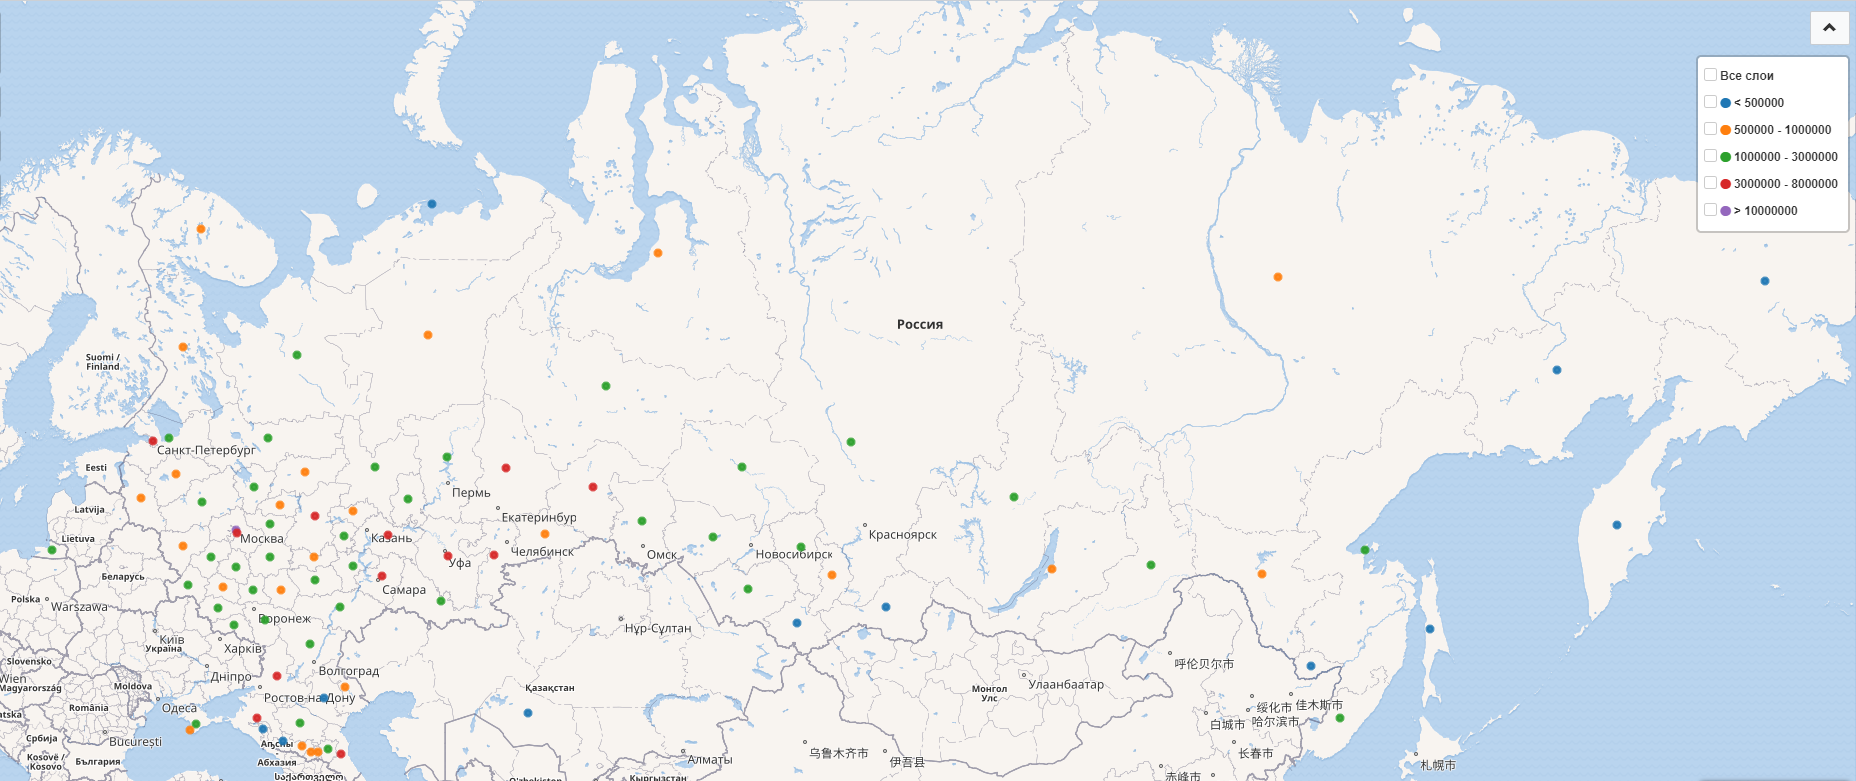
\includegraphics[width=1.0\linewidth]{./chapter/oblast_of_Russia/SubjectsRussia_Map_with_legend_RU.png}
	\caption[Map of the population by subjects of Russia, 2021.]{Population map by subjects of Russia, 2021. The subjects are divided into six groups by population and marked with different colors depending on the group the subject belongs to. The map is based on the data received by the request~\protect\ref{lst:map}.}%
      \label{fig:SubjectsRussiaMap}%
\end{figure*} 
%\end{fullwidth}

\newpage
\section{Page protection}

Wikidata pages are protected to prevent repeated vandalism or spam.

\begin{marginfigure}[1.0cm]
{
	\setlength{\fboxsep}{0pt}%
	\setlength{\fboxrule}{1pt}%
	{
\includegraphics[width=0.3\linewidth]{"chapter/oblast_of_Russia/Semi_protect.png"}}
}
\caption [Icon. Partial defense or midfield.]{Partial defense or midfield.}%
\label{fig:legend_population}%
\end{marginfigure}

\begin{marginfigure}[3.5cm]
{
	\setlength{\fboxsep}{0pt}%
	\setlength{\fboxrule}{1pt}%
	{
\includegraphics[width=0.3\linewidth]{"chapter/oblast_of_Russia/Full_protect.png"}}
	{
\includegraphics[width=0.3\linewidth]{"chapter/oblast_of_Russia/Permanent_protect.png"}}
}
\caption [Icon. Full protection.]{Full protection.}%
\label{fig:legend_population}%
\end{marginfigure}

\begin{marginfigure}[6.0cm]
{
	\setlength{\fboxsep}{0pt}%
	\setlength{\fboxrule}{1pt}%
	{
\includegraphics[width=0.3\linewidth]{"chapter/oblast_of_Russia/Move_protect.png"}}
}
\caption [Icon. Protection against renaming.]{Rename protection.}%
\label{fig:legend_population}%
\end{marginfigure}

\begin{marginfigure}[8.5cm]
{
	\setlength{\fboxsep}{0pt}%
	\setlength{\fboxrule}{1pt}%
	{
\includegraphics[width=0.3\linewidth]{"chapter/oblast_of_Russia/Create_protect.png"}}
}
\caption [Icon. Protection from creation.]{Creation protection.}%
\label{fig:legend_population}%
\end{marginfigure}

\begin{marginfigure}[11.0cm]
{
	\setlength{\fboxsep}{0pt}%
	\setlength{\fboxrule}{1pt}%
	{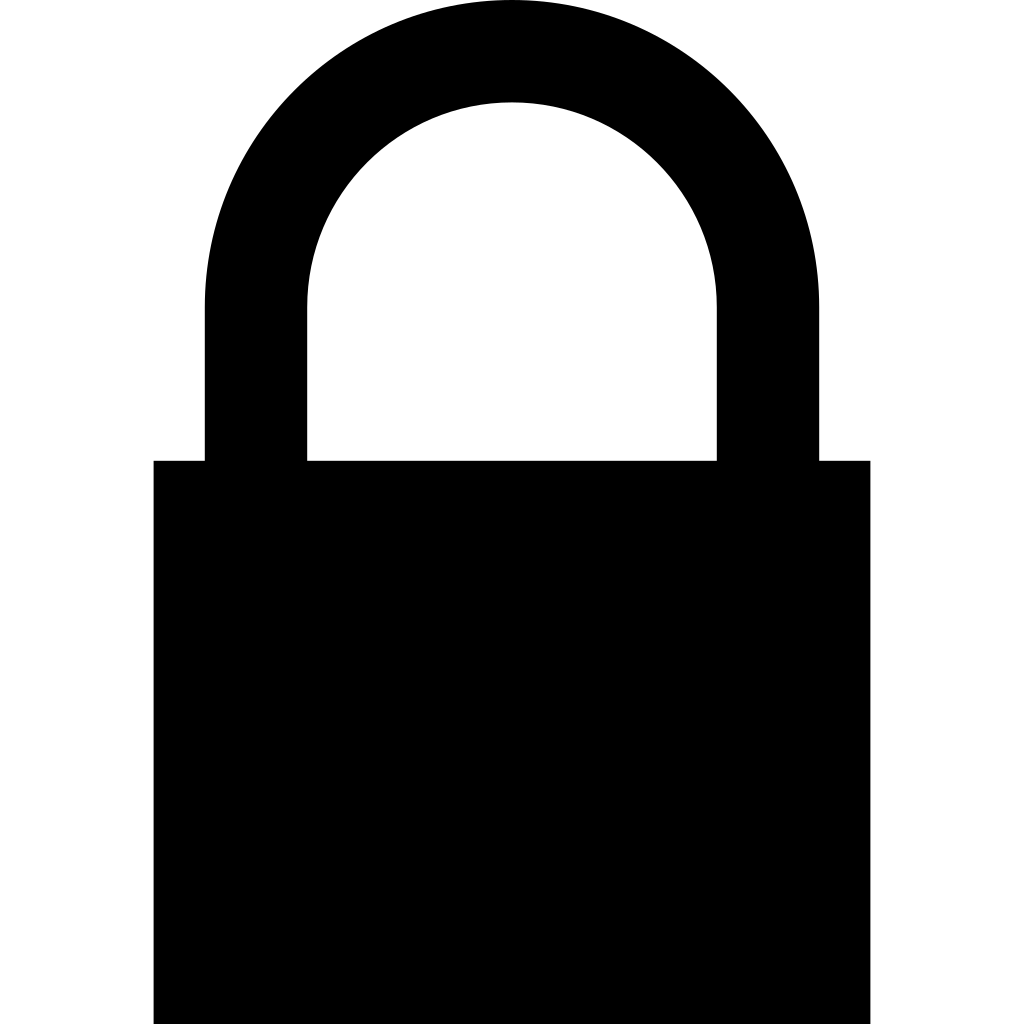
\includegraphics[width=0.3\linewidth]{"chapter/oblast_of_Russia/Office_action.png"}}
}
\caption [Icon. Official action.]{Official action.}%
\label{fig:legend_population}%
\end{marginfigure}

There are several types of protection:
\begin{itemize}
\item Partial protection or half-protection (indicated by a gray lock) allows only auto-confirmed/confirmed participants to edit the page.
  \item Full protection (indicated by an orange or red lock) limits the circle of editors to administrators.
  \item Renaming protection (indicated by a green lock) does not limit the ability to edit the page, but only administrators can rename it. Most popular pages are protected from renaming. Rename protection cannot be applied to element or property pages.
  \item Creation protection (both full and partial protection is indicated by a blue lock) can be applied to deleted or non-existent pages. However, like rename protection, it cannot be applied to deleted elements or properties.
  \begin{itemize}
	\item With full protection from creation, no one can create a page except administrators.
	\item With partial protection from creation, the page can also be created by auto-confirmed and confirmed participants.
  \end{itemize}
\end{itemize}

In extremely rare cases, the Wikimedia Foundation can protect a page as an official action (\textit{office action}, indicated by a black lock). Official actions are carried out only as a result of a formal non-media complaint, are always publicly announced and are carried out only by employees of the Wikimedia Foundation or members of the Board of Trustees.

Wikidata documentation contains additional materials about the protection of pages\protect\footnotemark
\footnotetext{See. page protection rules \href{https://goo-gl.me/OkHtF}{https://goo-gl.me/OkHtF}.}.